\documentclass[14pt, a4paper]{article}
\usepackage{minitoc}
\usepackage[left=3.00cm, right=2.5cm, top=2.00cm, bottom=2.00cm]{geometry}
\usepackage{amsmath}
\usepackage{amssymb}
\usepackage{amsthm}
\usepackage{mathtools}
\usepackage{graphicx}
%\usepackage{algpseudocode}
%\usepackage{algorithm}
\usepackage[ruled,vlined,linesnumbered]{algorithm2e}
\usepackage{blindtext}
\usepackage{setspace}
\usepackage[utf8]{inputenc}
\usepackage[utf8]{vietnam}
\usepackage[center]{caption}
\usepackage[shortlabels]{enumitem}
\usepackage{fancyhdr} % header, footer
\usepackage{hyperref} % loại bỏ border với mục lục và công thức
\usepackage[nonumberlist, nopostdot, nogroupskip]{glossaries}
\usepackage{glossary-superragged}
\usepackage{tikz,tkz-tab}
\usepackage{pythonhighlight}
\setglossarystyle{superraggedheaderborder}
\pagestyle{fancy}
%\usepackage[style=numeric,sortcites]{biblatex}
%\addbibresource{ref.bib}
%\usepackage[numbers]{natbib}
\usepackage{indentfirst}
\usepackage[natbib,backend=biber,style=ieee, sorting=ynt]{biblatex}
\bibliography{ref.bib}

\graphicspath{{./figures/}}

\fancyhf{}
\rhead{\textbf{Môn học: Toán rời rạc và thuật toán}}
\lhead{\textbf{GVHD: PGS. TS. Nguyễn Thị Hồng Minh}}
\rfoot{\thepage}
\lfoot{\textbf{Nhóm học viên thực hiện: Nhóm 01 - Cao học Khoa học dữ liệu - K4}}
\renewcommand{\headrulewidth}{0.4pt}
\renewcommand{\footrulewidth}{0.4pt}
%
%\numberwithin{equation}{section}
%\numberwithin{algorithm}{section}
%\numberwithin{figure}{section}
%
%\setlength{\parindent}{0.5cm}
%
%\setcounter{secnumdepth}{3} % Cho phép subsubsection trong report
%\setcounter{tocdepth}{3} % Chèn subsubsection vào bảng mục lục

%\newtheorem{dl}{Định lý}
%\newtheorem{md}{Mệnh đề}
%\newtheorem{bd}{Bổ đề}
%\newtheorem{dn}{Định nghĩa}
%\newtheorem{hq}{Hệ quả}

%\newtheorem{baitap}{Bài tập}
%\newtheorem*{loigiai}{Lời giải}

%\numberwithin{dl}{section}
%\numberwithin{md}{section}
%\numberwithin{bd}{section}
%\numberwithin{dn}{section}
%\numberwithin{hq}{section}

\setlength{\parindent}{0cm}

\newtheorem{dl}{Định lý}
\newtheoremstyle{sltheorem}
{}                % Space above
{}                % Space below
{\normalfont}        % Theorem body font % (default is "\upshape")
{}                % Indent amount
{\bfseries}       % Theorem head font % (default is \mdseries)
{.}               % Punctuation after theorem head % default: no punctuation
{ }               % Space after theorem head
{}                % Theorem head spec
\theoremstyle{sltheorem}
\newtheorem{baitap}{Bài tập}
\newtheoremstyle{soltheorem}
{}                % Space above
{}                % Space below
{\normalfont}        % Theorem body font % (default is "\upshape")
{}                % Indent amount
{\bfseries}       % Theorem head font % (default is \mdseries)
{.}               % Punctuation after theorem head % default: no punctuation
{\newline}               % Space after theorem head
{}                % Theorem head spec
\theoremstyle{soltheorem}
\newtheorem*{loigiai}{Lời giải}

\onehalfspacing

\begin{document}

    \begin{titlepage}

        \newcommand{\HRule}{\rule{\linewidth}{0.5mm}} % Defines a new command for the horizontal lines, change thickness here

        \center % Center everything on the page

        %----------------------------------------------------------------------------------------
        %	HEADING SECTIONS
        %----------------------------------------------------------------------------------------
        \textsc{\LARGE Đại học Quốc Gia Hà Nội}\\[0.5cm]
        \textsc{\LARGE Trường đại học Khoa học tự nhiên}\\[0.5cm] % Name of your university/college
        \textsc{\LARGE Khoa Toán - Cơ - Tin học}\\[0.5cm]

        
\includegraphics[scale=0.2]{HUS-logo.jpg}\\[0.5cm]

        \textsc{\Large Chuyên ngành: Khoa học dữ liệu}\\[0.5cm] % Major heading such as course name


        %----------------------------------------------------------------------------------------
        %	TITLE SECTION
        %----------------------------------------------------------------------------------------

        \HRule \\[0.4cm]
        { \huge \bfseries Bài tập môn học}\\[0.4cm] % Title of your document
        \HRule \\[1.5cm]

        \textsc{\Large Môn học: Toán rời rạc và thuật toán}\\[1cm] % Minor heading such as course title


        \textsc{\Large Bài tập 1: Các khái niệm cơ bản về thuật toán \\ và các phương pháp thiết kế thuật toán}\\[1cm]


        %----------------------------------------------------------------------------------------
        %	AUTHOR SECTION
        %----------------------------------------------------------------------------------------
        \begin{minipage}{0.4\textwidth}
            \begin{flushleft} \large
            \emph{Giảng viên hướng dẫn:} \\
            PGS. TS. Nguyễn Thị Hồng Minh % Supervisor's Name
            \end{flushleft}
        \end{minipage}\\[0.5cm]

        \begin{minipage}{0.4\textwidth}
        \begin{flushleft} \large
        \emph{Nhóm học viên thực hiện:}\\
        Nguyễn Chí Thanh \\
        MSHV: 21007925 \\ % Your name
        Vũ Ngọc Đại \\
        MSHV: 21007977 \\
        Vũ Minh Hưng \\
        MSHV: 21007973 \\
        Lê Diệu Thúy \\
        MSHV: 21007922 \\
        Lớp: Khoa học dữ liệu - K4
        \end{flushleft}
        \end{minipage}


        % If you don't want a supervisor, uncomment the two lines below and remove the section above
        %\Large \emph{Author:}\\
        %John \textsc{Smith}\\[3cm] % Your name

        %----------------------------------------------------------------------------------------
        %	DATE SECTION
        %----------------------------------------------------------------------------------------

        % I don't want day because it is English
        % {\large \today}\\[2cm] % Date, change the \today to a set date if you want to be precise

        %----------------------------------------------------------------------------------------
        %	LOGO SECTION
        %----------------------------------------------------------------------------------------

        %\includegraphics{logo/rsz_3logo-khtn.png}\\[1cm] % Include a department/university logo - this will require the graphicx package

        %----------------------------------------------------------------------------------------

        \vfill % Fill the rest of the page with whitespace

    \end{titlepage}

    \nocite{*}

    \newpage

    \begin{baitap}
        Hãy trình bày nhận thức, hiểu biết về vấn đề "Giải bài toán bằng thuật toán".
    \end{baitap}

    \begin{loigiai}

        \begin{enumerate}[a)]
            \item Bài toán và giải bài toán:
            Bài toán là bất cứ vấn đề nào cần được giải quyết. Trong tin học, thuật ngữ “bài toán” là lớp các bài toán cụ thể cùng loại mà ta cần máy tính thực hiện để có được kết quả.

            Có 2 yếu tố cần được đưa ra khi xác định bài toán:
            \begin{itemize}
                \item Thông tin đầu vào (input) là dữ liệu đã có
                \item Thông tin đầu ra (output): Những yếu tố cần xác định
            \end{itemize}
            $\Rightarrow$ Khi đó, cho bài toán tức là cho input và ouput. Khi phát biểu một bài toán, ta cần trình bày rõ Input và Output của bài toán đấy và mối quan hệ giữa chúng.
            
            Giải bài toán: từ input, dùng một số hữu hạn các bước thao tác có cơ sở toán học thích hợp để tìm được output theo yêu cầu của bài toán đề ra.

            Ví dụ 1: Xếp hạng các học viên trong lớp

            Input: Bảng điểm của các học sinh

            Output: Bảng xếp loại học lực

            Ví dụ 2: Giải phương trình bậc hai

            \begin{equation*}
                a x^2 + bx + c = 0 (a \neq 0)
            \end{equation*}

            Input: Các số thực $a, b, c (a \neq 0)$

            Output: Các số thực $x$ thỏa mãn $ax^2 + bx + c = 0$

            Ở bài toán này, ta có thể đưa ra kết quả bài toán là 2 số thực thoả mã điều kiện hoặc phương trình vô nghiệm

            Ví dụ 3: Tính diện tích hình tròn $\mathcal{C}$

            Input: Bán kính hình tròn $\mathcal{C}$ và công thức tính diện tích hình tròn

            Output: Diện tích hình tròn $\mathcal{C}$

            Ví dụ 4: Tìm đường đi ngắn nhất từ $u$ đến $v$ của đồ thị $G=(V, E)$

            Input: Đồ thị $G$

            Output: Xác định đường đi $d=(u=v_1, v_2, \dots, v_n=n)$ (với $v_i \in V$, $(v_i, v_{i + 1}) \in E$) có độ dài ngắn nhất
            \item Thuật toán (Algorithms)
            \begin{itemize}
                \item Khái niệm cơ bản:
                
                Thuật toán là một dãy hữu hạn các thao tác đơn giản được sắp xếp theo một trình tự xác định dùng để giải một bài toán.

                Ta cũng có thể hiểu thuật toán là tập hợp hữu hạn các quy tắc ta sử dụng để có thể có được đầu ra mong đợi từ đầu vào đã cho ban đầu.

                \begin{figure}[h!]
                    \centering
                    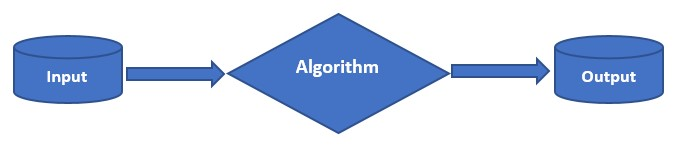
\includegraphics[scale=0.6]{algorithm.jpg}
                    \caption{Minh họa một thuật toán}
                \end{figure}

                \item Một số phương pháp diễn đạt thuật toán:
                \begin{itemize}
                    \item Liệt kê từng bước theo ngôn ngữ tự nhiên hàng ngày. 
                    \item Sơ đồ khối (flowchart). Lưu ý phân biệt Thao tác chọn lựa (decision) và Thao tác xử lý (process). Chẳng hạn : thao tác "nếu $a=b$ thì thực hiện thao tác B2, nếu $a \neq b$ thực hiện B4" là thao tác chọn lựa. Các thao tác còn lại không thuộc loại chọn lựa được xếp vào loại hành động. Chẳng hạn, "Chọn một hộp bất kỳ và để lên dĩa cân còn trống." là một thao tác thuộc loại hành động.
                    \begin{figure}[h!]
                        \centering
                        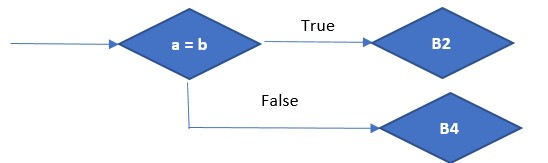
\includegraphics[scale=0.8]{flowchart.jpg}
                        \caption{Ví dụ minh họa sơ đồ khối}
                    \end{figure}
                    \item Mã giả (pseudo-code). Vẫn sử dụng 1 phần ngôn ngữ tự nhiên. Nhưng vì các thuật toán thường có các thao tác lặp nên mã giả hay vay mượn cú pháp của các ngôn ngữ lập trình để thể hiện cho tường minh.
                    \begin{algorithm}
                        \DontPrintSemicolon
                        \KwIn{$a, b, c (a \neq 0)$}
                        \KwOut{Nghiệm nếu có của phương trình bậc 2}
                        $\Delta \gets \dfrac{b^2 - 4ac}{2a}$\;
                        \If{$\Delta > 0$} {
                            $x_1 \gets \dfrac{-b + \sqrt{\Delta}}{2a}$\;
                            $x_2 \gets \dfrac{-b - \sqrt{\Delta}}{2a}$\;
                            \Return{$x_1, x_2$}\;
                        } \Else {
                            \If {$\Delta = 0$} {
                                $x_1 = x_2 \gets \dfrac{-b}{2a}$\;
                                \Return {$x_1, x_2$}\;
                            } \Else {
                                Phương trình vô nghiệm \;
                            }
                        }
                        \caption{Mã giả thuật toán giải phương trình bậc 2}
                    \end{algorithm}  
                \end{itemize}
                \item Phân tích để đánh giá thuật toán.
                
                Chúng ta thường có xu hướng chọn cách giải "tốt nhất", hoặc thuật toán "tốt nhất" cho 1 bài toán. 
                Để đánh giá thế nào là "tốt nhất", chúng ta có thể dựa vào 1 số tiêu chí sau: Thuật toán có đơn giản, dễ hiểu, dễ cài đặt hay không? 
                Thuật toán có hiệu quả hay không dựa vào hai yếu tố là thời gian thực hiện thuật toán (còn gọi là độ phức tạp thuật toán) và tài nguyên sẽ được sử dụng khi thuật toán thi hành (còn gọi là độ phức tạp không gian). 
                Tuy nhiên, trong bối cảnh hiện tại khi các máy tính có khả năng lưu trữ rất lớn thì yếu tố mà chúng ta cần quan tâm nhiều hơn là độ phức tạp thời gian thuật toán.
                \begin{itemize}
                    \item Độ phức tạp của thuật toán
                    Thời gian thực hiện thuật toán (running time) là số các thao tác cơ bản được thực hiện: phép tính số học, logic cơ bản hoặc một câu lệnh "đơn"...
                    
                    Các phương pháp đánh giá thời gian thực hiện thuật toán:
                    \begin{itemize}
                        \item Phương pháp thực nghiệm: Chúng ta lập trình, định nghĩa các thuật toán, chạy thử nhiệm, ghi nhận các số đo về độ phức tạp.
                        
                        Ưu điểm: Có thể đánh giá được tất cả các thuật toán khả trình theo số liệu thực tế trả về.

                        Nhược điểm: Kết quả đánh giá có thể có sai số và phụ thuộc vào máy tính thực hiện, môi trường thực hiện, thời điểm thực hiện.

                        \item Phương pháp lý thuyết: Xác định quan hệ về thời gian với kích thước dữ liệu bằng hàm toán học. Trong phương pháp này, ta quan tâm tới yêu tố kích thước của dữ liệu đầu vào, thông thường là một con số n. Mối liên hệ giữa yếu tố này và số lượng các phép tính toán để tìm ra được kết quả của bài toán gọi là độ phức tạp thuật toán (kết quả của nó không phải được tính bằng thời gian như 1, 2 hay bao nhiêu giây).
                        
                        Ưu điểm: không phụ thuộc ngôn ngữ lập trình, loại máy tính; đánh giá được với dữ liệu có kích thước lớn.

                        Nhược điểm: Khó thực hiện hơn vì phải biểu diễn các ràng buộc về mặt toán học

                        Ví dụ: Tính tổng các số nguyên từ $1$ đến $n$. Dùng công thức $\dfrac{n (n + 1)}{2}$. Giải thuật này có độ phức tạp là $O(1)$ (1 phép toán).
                        Bài toán kiểm tra số nguyên tố. Nếu kiểm tra từ $1$ đến $n$, độ phức tạp là $O(n)$. Nếu chạy từ $1$ đến $\sqrt{n}$ thì đã giảm rất nhiều phép toán.
                    \end{itemize}
                \end{itemize}
                \item Một số thuật toán
                
                \begin{itemize}
                    \item Các thuật toán sắp xếp (Sort Algorithms)
                    \begin{itemize}
                        \item Bubble Sort
                        \item Selection Sort
                        \item Insertion Sort
                        \item Quick Sort
                        \item Merge Sort
                        \item Heap Sort
                    \end{itemize}
                    \item Các thuật toán tìm kiến (Search Algorithms)
                    \begin{itemize}
                        \item BFS (Breadth-first search): Thuật toán tìm kiếm theo chiều rộng là một thuật toán tìm kiếm trong đồ thị trong đó việc tìm kiếm chỉ bao gồm 2 thao tác: (a) cho trước một đỉnh của đồ thị; (b) thêm các đỉnh kề với đỉnh vừa cho vào danh sách có thể hướng tới tiếp theo.
                        \item Binary search: là một thuật toán tìm kiếm xác định vị trí của một giá trị cần tìm trong một mảng đã được sắp xếp. Chi phí trong trường hợp tốt nhất $O(1)$, chi phí trong trường hợp trung bình $O(\log n)$
                    \end{itemize}
                \end{itemize}
            \end{itemize}
            \item Giải bài toán bằng thuật toán
            Một thuật toán cũng giống như một bản kế hoạch để giải quyết một bài toán. Việc phát triển thuật toán là một bước then chốt để giải quyết vấn đề. Quy trình phát triển thuật toán nói chung thường bao gồm 5 bước chính sau:
            \begin{enumerate}[1.]
                \item Thu thập mô tả về bài toán:
                \begin{itemize}
                    \item Bước này thường liên quan đến việc trao đổi thông tin giữa bên đưa ra bài toán (client) và bên có trách nhiệm giải quyết bài toán (developer). Và thường đây là bước yếu nhất trong toàn bộ quy trình. Thông thường bước này sẽ xảy ra các thiếu sót như sau:
                    \begin{itemize}
                        \item Các mô tả dựa trên những giả định ngầm
                        \item Mô tả không rõ ràng
                        \item Mô tả không đẩy đủ
                        \item Mô tả có sự mâu thuẫn lẫn nhau
                    \end{itemize}
                    \item Nhiệm vụ của người chịu trách nhiệm giải quyết bài toán là phải phát hiện ra những thiếu sót trong mô tả của bài toán và phối hợp với bên đưa ra bài toán để giải quyết những thiếu sót này.
                \end{itemize}
                \item Phân tích bài toán:
                \begin{itemize}
                    \item Mục tiêu của bước này là xác định các điểm bắt đầu và kết thúc của bài toán.
                    \item Khi xác định điểm bắt đầu, ta nên trả lời những câu hỏi sau:
                    \begin{itemize}
                        \item Những dự kiện nào đang có?
                        \item Dữ kiện đó nằm ở đâu?
                        \item Công thức liên quan tới bài toán là gì?
                        \item Mối quan hệ giữa các dữ kiện?
                    \end{itemize}
                    \item Khi xác định điểm kết thúc, ta cần biết khi nào thì kết thúc bài toán. Và trả lời những câu hỏi sau sẽ giúp xác định điểm kết thúc:
                    \begin{itemize}
                        \item Ta sẽ có thêm những thông tin gì?
                        \item Những dữ kiện nào đã thay đổi?
                        \item Những thay đổi đó là gì?
                        \item Những dữ kiện nào đã biến mất?
                    \end{itemize}
                \end{itemize}
                \item Phát triển một thuật toán ở mức sơ lược
                \begin{itemize}
                    \item Một thuật toán là một kế hoạch để giải quyết bài toán, nhưng kế hoạch sẽ có nhiều mức chi tiết khác nhau. Thường ta nên bắt đầu với một thuật toán ở mức sơ lược mà chỉ bao gồm những phần trọng yếu cho bài toán.
                    \item Những chi tiết sẽ được bổ sung thêm ở bước tiếp theo của quy trình.
                \end{itemize}
                \item Tinh chỉnh thuật toán bằng cách bổ sung thêm các chi tiết
                \begin{itemize}
                    \item Thuật toán sơ lược ở bước trước chỉ bao gồm những thành phần chính để giải quyết bài toán. Giờ ta cần bổ sung thêm các chi tiết cho lời giải, và mức độ chi tiết thì cần tùy thuộc vào từng tình huống.
                    \item Nếu bài toán cần giải quyết mà phức tạp, thì bước tinh chỉnh, bổ sung này sẽ cần phải lặp lại vài lần. Ở mỗi lần bổ sung, ta thêm các chi tiết mới vào thuật toán trước đó, và chỉ dừng lại khi không còn thấy lợi ích của việc tinh chỉnh.
                \end{itemize}
                \item Đánh giá lại thuật toán
                \begin{itemize}
                    \item Ở bước này, ta cần đi qua toàn bộ thuật toán từng bước một để xác định liệu bước đó sẽ giúp dẫn đến câu trả lời cho bài toán. Một khi xác định được rằng thuật toán đã giải được bài toán, ta cần xem xét thêm các yếu tố khác. Một số yếu tố đó bao gồm:
                    \begin{itemize}
                        \item Thuật toán này giải quyết một bài toán cá biệt hay giải quyết một bài toán tổng quát?
                        \item Thuật toán có thể được đơn giản hơn hay không? Ví dụ: một công thức tính chu vi của hình chữ nhật sẽ như sau:
                        \begin{equation*}
                            C=length+width+length+width
                        \end{equation*}
                        Một lời giải tối ưu hơn sẽ như sau:
                        \begin{equation*}
                            C = 2 \times (length + width)
                        \end{equation*}
                        \item Lời giải này có tương tự lời giải cho một bài toán khác không? Chúng giống hoặc khác nhau như thế nào?
                    \end{itemize}
                    \item Và đến đây, ta đã hoàn thành xong bước cuối cùng của quy trình giải một bài toán bằng thuật toán.
                \end{itemize}
            \end{enumerate}
        \end{enumerate}
    \end{loigiai}

    \begin{baitap}
        Trình bày các vấn đề liên quan tới một trong các phương pháp cơ bản thiết kế
        thuật toán sau: \textbf{chia để trị, quay lui, quy hoạch động}. Các nội dung trình bày bao gồm:
        \begin{itemize} [label={$-$}]
            \item Ý tưởng của phương pháp thiết kế thuật toán.
            \item Các nội dung để thiết kế và đánh giá thuật toán: mô hình, lược đồ, phân tích…
            \item Bài toán ví dụ: phát biểu bài toán, thiết kế thuật toán, đánh giá thuật toán
            bằng lí thuyết, bằng thực nghiệm.
        \end{itemize}
    \end{baitap}

    \begin{loigiai}
        Các nội dung cơ bản của phương pháp quy hoạch động:

        \textbf{Ý tưởng của phương pháp quy hoạch động:}

        Như ta đã biết, các thuật toán đệ quy có ưu điểm là dễ thực thi nhưng do bản chất của quá trình thực hiện đệ quy,
        các chương trình thường kéo theo chi phí lớn về cả bộ nhớ và tính toán.

        Quy hoạch động (dynamic programming) là một phương pháp nhằm làm đơn giản việc tính toán các công thức truy hồi bằng cách lưu toàn bộ hay một phần kết quả tại mỗi bước với mục đích sử dụng lại.
        Từ "programming" trong "dynamic programming" không có ý nghĩa là việc lập trình cho máy tính,
        mà là một thuật ngữ mà các nhà toán học hay các nhà khoa học máy tính dùng để đưa ra các bước chung trong việc giải quyết một lớp các bài toán.
        Tuy nhiên không có một thuật toán tổng quát nào để giải tất cả các bài toán quy hoạch động.

        Quy hoạch động giúp giải quyết rất hiệu quả các lớp bài toán mà có các bài toán con gối nhau và có cấu trúc con tối ưu.
        Những bài toán có dạng này liên quan đến việc tính toán nhiều lần giá trị của các bài toán con giống hệt nhau để tìm ra giải pháp tối ưu.

        \begin{itemize}
            \item Các bài toán con gối nhau: Bài toán con là các bài toán nhỏ hơn của bài toán ban đầu.
            Bất kỳ một bài toán nào được giải cũng có các bài toán con trùng nhau nếu việc tìm lời giải của bài toán liên quan đến việc giải cùng một bài toán con nhiều lần.

            \item Cấu trúc con tối ưu: Bất kỳ bài toán nào cũng có cấu trúc con tối ưu nếu lời giải tối ưu tổng thể của bài toán này được xây dựng từ các lời giải tối ưu của các bài toán con của nó.
        \end{itemize}

        Phương pháp quy hoạch động dùng để giải bài toán tối ưu có bản chất đệ quy, tức là việc tìm
        phương án tối ưu cho bài toán đó có thể đưa về tìm phương án tối ưu của một số hữu hạn các bài toán con.
        Hoặc phương pháp quy hoạch động cũng có thể được sử dụng để giải các bài toán có bản chất đệ quy mà các bài toán con được gọi nhiều lần.

        Đối với nhiều thuật toán đệ quy đã biết, phương pháp chia để trị đóng vai trò chủ đạo trong việc thiết kế thuật toán.
        Để giải quyết một bài toán lớn, ta chia bài toán này làm nhiều bài toán con cùng dạng với nó để có thể giải quyết độc lập.
        Những bài toán con này lại được chia thành những bài toán con nhỏ hơn nữa, ... đến lúc đạt được bài toán đủ đơn giản để có thể giải trực tiếp được.
        Sau đó nghiệm của những bài toán con được tổng hợp lại theo một phương pháp thích hợp để thu được lời giải của bài toán ban đầu.
        Khác với phương pháp chia để trị, phương pháp quy hoạch động không yêu cầu các bài toán con phải không giao nhau.

        Phép phân rã đệ quy bắt đầu từ bài toán lớn phân rã thành nhiều bài toán con và đi giải từng bài toán con đó.
        Việc giải từng bài toán con lại đưa tiếp về phép phân rã thành nhiều bài toán nhỏ hơn và lại đi giải bài toán nhỏ hơn đó bất kể nó đã được giải hay chưa.

        Ngược lại, phương pháp quy hoạch động bắt đầu từ việc giải tất cả các bài toán con nhỏ nhất và lưu lại lời giải của từng bài toán con này
        để từng bước giải quyết những bài toán lớn hơn cho đến khi giải được bài toán lớn nhất.

        Để xem phương pháp quy hoạch động có thể sử dụng để giải một bài toán, ta cần xem xét bài toán có những tính chất sau đây hay không:


        \begin{itemize}
            \item Bài toán lớn phải phân rã được thành nhiều bài toán con, mà sự phối hợp lời giải của các bài
            toán con đó cho ta lời giải của bài toán lớn. 
            \item Vì quy hoạch động là đi giải tất cả các bài toán con, nên nếu không đủ không gian vật lý lưu
            trữ lời giải (bộ nhớ, đĩa…) để phối hợp chúng thì phương pháp quy hoạch động cũng không
            thể thực hiện được. 
            \item Quá trình từ bài toán cơ sở tìm ra lời giải bài toán ban đầu phải qua hữu hạn bước.
        \end{itemize}

        Các bước để giải một bài toán bằng phương pháp quy hoạch động:

        \begin{itemize}
            \item Giải tất cả các bài toán cơ sở, lưu các lời giải vào bảng phương án.
            \item Dùng công thức truy hồi phối hợp những lời giải của những bài toán nhỏ đã lưu trong bảng
            phương án để tìm lời giải của những bài toán lớn hơn và lưu chúng vào bảng phương án. Cho
            tới khi bài toán ban đầu tìm được lời giải.
            \item Dựa vào bảng phương án, truy vết tìm ra nghiệm tối ưu.
        \end{itemize}

        Bước xác định công thức truy hồi giữa các bài toán là bước khó nhất và quan trọng nhất.
        Đến nay vẫn chưa có một định lý nào cho biết một cách chính xác những bài toán nào có thể giải quyết hiệu quả bằng phương pháp quy hoạch động.
        Tuy nhiên để biết được bài toán có thể giải bằng
        quy hoạch động hay không, ta có thể tự đặt câu hỏi: "Một nghiệm tối ưu của bài toán lớn có
        phải là sự phối hợp các nghiệm tối ưu của các bài toán con hay không?" và ”Liệu có thể
        nào lưu trữ được nghiệm các bài toán con dưới một hình thức nào đó để phối hợp tìm
        được nghiệm bài toán lớn hay không?"

        So sánh phương pháp chia để trị với phương pháp quy hoạch động:

        \begin{itemize}
            \item Phương pháp chia để trị là kết hợp lời giải của các bài toán con để tìm ra lời giải của bài toán ban đầu.
            \item Phương pháp quy hoạch động là sử dụng kết quả của bài toán con và sau đó cố gắng tối ưu bài toán lớn hơn.
            Phương pháp quy hoạch động sử dụng phương pháp lưu trữ để ghi nhớ kết quả của các bài toán con đã được giải.
        \end{itemize}

        So sánh phương pháp tham lam với phương pháp quy hoạch động:

        \begin{itemize}
            \item Phương pháp tham làm là một phương pháp tìm kiếm, lựa chọn giải pháp tối ưu địa phương ở mỗi bước với hy vọng tìm được giải pháp tối ưu toàn cục.
            \item Phương pháp quy hoạch động tối ưu hóa các bài toán con gối nhau.
        \end{itemize}

        \textbf{Các bài toán ví dụ:}

        \begin{itemize} [label={$-$}]
            \item \textbf{Ví dụ 1:}
            Cho hai xâu $\bold{X}$ và $\bold{Y}$. Xâu gốc có $n$ ký tự $\bold{X} \lbrack 1 \rbrack, \bold{X} \lbrack 2 \rbrack, \dots, \bold{X} \lbrack n \rbrack$, xâu đích có $m$ ký tự $\bold{Y} \lbrack 1 \rbrack, \bold{Y} \lbrack 2 \rbrack, \dots, \bold{Y} \lbrack m \rbrack$.
            Có 3 phép biến đổi:
            \begin{itemize} [label={$+$}]
                \item Chèn một ký tự vào sau ký tự thứ $i$
                \item Thay thế ký tự ở vị trí thứ $i$ bằng ký tự $C$
                \item Xóa ký tự ở vị trí thứ $i$
            \end{itemize}
            Hãy tìm số ít nhất các phép biến đổi để biến xâu $\bold{X}$ thành xâu $\bold{Y}$

            \textbf{Đầu vào:}

            Dòng đầu tiên là xâu gốc
            Dòng thứ hai là xâu đích
            
            \textbf{Đầu ra:}

            Số phép biển đổi ít nhất để biến xâu gốc thành xâu đích
        %\end{itemize}

        Ta nhận thấy số phép biến đổi phụ thuộc vào vị trí $i$ đang xét của xâu gốc $\bold{X}$ và vị trí đang xét $j$ của xâu đích.
        Ta gọi $\bold{L}\lbrack i, j \rbrack$ là số phép biến đổi ít nhất để biến xâu $\bold{X}_i$ gồm $i$ ký tự đầu của xâu gốc $\bold{X}$ ($\bold{X}_i = \bold{X}\lbrack 1 \dots i \rbrack$)
        thành xâu $\bold{Y}_j$ gồm $j$ ký tự đầu của xâu đích $\bold{Y}$ ($\bold{Y}_j=\bold{Y} \lbrack 1 \dots j \rbrack$).
        
        Ta nhận thấy $\bold{L}\lbrack 0, j \rbrack=j$ và $\bold{L}\lbrack i, 0 \rbrack=i$

        Tại điểm $(i, j)$ của bảng phương án $\bold{L}$ có hai trường hợp xảy ra:

        \begin{itemize}
            \item Nếu $\bold{X} \lbrack i \rbrack = \bold{Y} \lbrack j \rbrack$: Ta chỉ cần biến đổi xâu $\bold{X}_{i-1}$ thành xâu $\bold{Y}_{j-1}$.
            Vì vậy $\bold{L}\lbrack i, j \rbrack = \bold{L}\lbrack i-1, j-1 \rbrack$
            \item Nếu $\bold{X} \lbrack i \rbrack \neq \bold{Y} \lbrack j \rbrack$, ta có ba cách biến đổi:
            \begin{itemize}
                \item Xóa ký tự $\bold{X} \lbrack i \rbrack$. Xâu $\bold{X}_{i-1}$ thành xâu $\bold{Y}_j$. Khi này $\bold{L}\lbrack i, j \rbrack=\bold{L} \lbrack i-1, j \rbrack + 1$.
                \item Thay thế ký tự $\bold{X} \lbrack i \rbrack$ thành ký tự $\bold{Y} \lbrack j \rbrack$.
                Trước đấy ta cần biến đổi xâu $\bold{X}_{i-1}$ thành xâu $\bold{Y}_{j-1}$. Khi này $\bold{L} \lbrack i, j \rbrack = \bold{L} \lbrack i-1, j-1 \rbrack + 1$.
                \item Thêm ký tự $\bold{Y} \lbrack j \rbrack$ vào sau xâu $\bold{X}_i$. Trước đấy ta cần biến đổi xâu $\bold{X}_{i}$ thành xâu $\bold{Y}_{j-1}$.
                Khi này $\bold{L} \lbrack i, j \rbrack = \bold{L} \lbrack i, j-1 \rbrack + 1$
            \end{itemize}
        \end{itemize}

        Tổng hợp các công thức trên lại, ta có công thức tính các phần tử của bảng phương án $\bold{L}$:

        \begin{equation*}
            \bold{L} \lbrack i, j \rbrack = \begin{cases} j ,\text{ nếu } i = 0 \\
            i , \text{ nếu } j = 0 \\
            \bold{L} \lbrack i-1, j-1 \rbrack, \text{ nếu } \bold{X} \lbrack i \rbrack = \bold{Y} \lbrack j \rbrack \\
            \min \Big ( \bold{L} \lbrack i-1, j \rbrack, \bold{L} \lbrack i, j-1 \rbrack, \bold{L} \lbrack i-1, j-1 \rbrack + 1 \Big), \text{ nếu } \bold{X}\lbrack i \rbrack \neq \bold{Y} \lbrack j \rbrack \end{cases}
        \end{equation*}

        Sơ đồ mã giả thuật toán bài toán này là:

        \begin{algorithm}[h!]
            \DontPrintSemicolon
            \KwIn{Xâu gốc $\bold{X}$ gồm $n$ ký tự, xâu đích $\bold{Y}$ gồm $m$ ký tự}
            \KwOut{Số phép biến đổi ít nhất để biến xâu gốc $\bold{X}$ thành xâu đích $\bold{Y}$}
            Khởi tạo $\bold{L} \lbrack i, j \rbrack =0, \thickspace \forall \thickspace i=\overline{0, n}, j=\overline{0,m}$\;
            \For{$i \gets 0$ \textbf{to} $n$} {
                \For{$j \gets 0$ \textbf{to} $m$} {
                    \If{$i = 0$}
                    {

                        $\bold{L} \lbrack i, j \rbrack \gets j$\;
                        continue\;
                    }
                    \If{$j = 0$}
                    {

                        $\bold{L} \lbrack i, j \rbrack \gets i$\;
                        continue\;
                    }
                    \If{$\bold{X} \lbrack i \rbrack = \bold{Y} \lbrack j \rbrack$}
                    {
                        $\bold{L} \lbrack i, j \rbrack \gets \bold{L} \lbrack i-1, j-1 \rbrack$\;
                    }
                    \Else 
                    {
                        $\bold{L} \lbrack i, j \rbrack \gets \min \Big ( \bold{L} \lbrack i-1, j \rbrack, \bold{L} \lbrack i, j-1 \rbrack, \bold{L} \lbrack i-1, j-1 \rbrack + 1 \Big)$\;
                    }
                }
            }
            \Return {$\bold{L} \lbrack n, m \rbrack$}\;
            \caption{Thuật toán tìm số cách nhỏ nhất để biến đổi xâu gốc $\bold{X}$ thành xâu đích $\bold{Y}$}
        \end{algorithm}

        Thuật toán trên gồm 2 vòng lặp lồng nhau. Độ phức tạp tính toán của thuật toán là $O(nm)$ và độ phức tạp về bộ nhớ của thuật toán là $O(nm)$ (lưu bảng phương án hai chiều $\bold{L}$). 
        Code của thuật toán trên được trình bày ở phụ lục \ref{code-1-ex-2}

        Thực nghiệm:

        \begin{itemize}
            \item Với đầu vào:
            \begin{verbatim}
                dkfjaldfas
                djflkafdas
            \end{verbatim}
            Kết quả đầu ra:
            \begin{verbatim}
                5
            \end{verbatim}
            Thời gian chạy: 0.00011999 (giây)
            \item Với đầu vào:
            \begin{verbatim}
                ueioqurwortuwotywo
                tiuwonglsjgowtjwoot
            \end{verbatim}
            Kết quả đầu ra:
            \begin{verbatim}
                15
            \end{verbatim}
            Thời gian chạy: 0.00042899 (giây)
        \end{itemize}

        Ta nhận thấy với kích thước (độ dài xâu) tăng gấp đôi thì thời gian chạy tăng khoảng 4 lần phù hợp với độ phức tạp tính toán trong lý thuyết $O(nm)$.

        \item \textbf{Ví dụ 2:} Cho hai xâu ký tự, xâu thứ nhất có độ dài $n$ và xâu thứ hai có độ dài $m$.
        Tìm xâu con chung có độ dài dài nhất giữa hai xâu trên.

        \textbf{Đầu vào:}
        Dòng đầu tiên là xâu thứ nhất

        Dòng thứ hai là xâu thứ hai

        \textbf{Đầu ra:}

        Xâu con chung của hai xâu có độ dài dài nhất

        Gọi xâu đầu tiên là $\bold{X}$, xâu thứ hai là $\bold{Y}$.
        Ta gọi $\bold{S} \lbrack i, j \rbrack$ là độ dài xâu con chung dài nhất kết thúc $i$ ký tự đầu của xâu thứ nhất và kết thúc tại $j$ ký tự đầu của xâu thứ hai.
        Ta có nhận xét:

        \begin{itemize}
            \item Nếu $i = 0 \text{ hoặc } j = 0$ thì $\bold{S} \lbrack i, j \rbrack=0$
            \item Nếu $\bold{X} \lbrack i \rbrack = \bold{X} \lbrack j \rbrack$ thì $\bold{S} \lbrack i, j \rbrack= \bold{S} \lbrack i - 1, j - 1 \rbrack + 1$.
            \item Nếu $\bold{X} \lbrack i \rbrack \neq \bold{Y} \lbrack j \rbrack $ thì $\bold{S} \lbrack i, j \rbrack = 0$
        \end{itemize}

        Từ lập luận trên, ta có công thức tổng quát tính giá trị các phần tử của $\bold{S}$:

        \begin{equation*}
            \bold{S} \lbrack i, j \rbrack = \begin{cases} 0 \text{ nếu } i = 0 \text{ hoặc } j = 0 \\ 
            \bold{S} \lbrack i - 1, j - 1 \rbrack + 1 \text{ nếu } \bold{X} \lbrack i \rbrack = \bold{Y} \lbrack j \rbrack \\
            0  \text{ nếu } \bold{X} \lbrack i \rbrack \neq \bold{Y} \lbrack j \rbrack  \end{cases}
        \end{equation*}

        Để truy vết xâu cong chung dài nhất, ta đặt một biến để lưu vị trí lớn nhất trong $\bold{S}$ và giá trị lớn nhất tương ứng.
        Sau khi tính hết các phần tử $\bold{S}$, từ vị trí và độ dài xâu con chung lớn nhất ta sẽ thu được xâu con chung dài nhất.

        Ta có thuật toán tìm xâu con chung dài nhất của hai xâu $\bold{X}$ và xâu $\bold{Y}$:

        \begin{algorithm}
            \DontPrintSemicolon
            \KwIn{Xâu $\bold{X}$ có độ dài $n$, xâu $\bold{Y}$ có độ dài $m$}
            \KwOut{Xâu con chung dài nhất của hai xâu $\bold{X}$ và xâu $\bold{Y}$}

            $max\_len \gets - \infty$\;
            \For{$i \gets 0$ \textbf{to} $n$} {
                \For {$j \gets 0$ \textbf{to} $m$} {
                    \If{$i = 0$ \textbf{or} $j = 0$} {
                        $\bold{S} \lbrack i, j \rbrack \gets 0$\;
                        \textbf{continue}\;
                    }
                    \If{$\bold{X} \lbrack i \rbrack = \bold{Y} \lbrack j \rbrack $} {
                        $\bold{S} \lbrack i, j \rbrack \gets \bold{S} \lbrack i - 1, j - 1 \rbrack + 1$\;
                        \If{$\bold{S} \lbrack i, j \rbrack > max\_len$} {
                            $max\_len \gets \bold{S} \lbrack i, j \rbrack$\;
                            $pos\_row \gets i$\;
                        }
                        \textbf{continue}\;
                    }
                    \If{$\bold{X} \lbrack i \rbrack \neq \bold{Y} \lbrack j \rbrack$} {
                        $\bold{S} \lbrack i, j \rbrack \gets 0$\;
                    }
                }
            }
            $longest\_substring \gets \bold{X} \lbrack pos\_row - max\_len + 1: pos\_row \rbrack$\;
            \Return{$longest\_substring$}\;
            \caption{Thuật toán tìm xâu con chung dài nhất của hai xâu $\bold{X}$ và xâu $\bold{Y}$}
        \end{algorithm}

        Thuật toán trên có 2 vòng lặp lồng nhau.
        Độ phức tạp tính toán của thuật toán là $O(nm)$ và độ phức tạp về bộ nhớ của thuật toán là $O(nm)$ (lưu bảng phương án hai chiều $\bold{S}$).
        Code của thuật toán trên được trình bày ở phụ lục \ref{code-2-ex-1}.

        Thực nghiệm:

        \begin{itemize}
            \item Với đầu vào:
            \begin{verbatim}
                fdajlkdfjagdjl
                akfdldfjkajlkd
            \end{verbatim}
            Kết quả đầu ra:
            \begin{verbatim}
                ajlkd
            \end{verbatim}
            Thời gian chạy: 0.000093029 (giây)
            \item Với đầu vào:
            \begin{verbatim}
                fhdjlsfjlafjlafjkdsfhksdfsfdk  
                fjkdlsflfsdjfjlafjlaruieowrwo
            \end{verbatim}
            Kết quả đầu ra:
            \begin{verbatim}
                fjlafjla
            \end{verbatim}
            Thời gian chạy: 0.00040400 (giây)
        \end{itemize}

        Ta nhận thấy với kích thước (độ dài xâu) tăng gấp đôi thì thời gian chạy tăng khoảng 4 lần phù hợp với độ phức tạp tính toán trong lý thuyết $O(nm)$.

        \item \textbf{Ví dụ 3:} Cho $n$ ma trận $\bold{A}_1, \bold{A}_2, \dots, \bold{A}_n$, ma trận $\bold{A}_i$ có kích thước $d_{i-1} \times d_i$.
        Hãy tính số phép tính nhỏ nhất để thực hiễn phép nhân $\bold{A}_1 \times \bold{A}_2 \times \dots \times \bold{A}_n$
        \textbf{Đầu vào:}
    
        Dòng đầu tiên ghi số nguyên dương $n$ là số ma trận
    
        Dầu thứ hai ghi $n+1$ số nguyên là kích thước của chuỗi ma trận
    
        \textbf{Đầu ra:}
    
        Một dòng ghi số phép tính nhỏ nhất khi thực hiện nhân chuỗi ma trận trên
    
        Ta nhận thấy kết quả của nhân hai ma trận $\bold{A}_i \bold{A}_{i + 1}$ là một ma trận có kích thước $d_{i-1} \times d_{i+1}$ ta cần số phép tính là: $d_{i-1} (2 d_i - 1) d_{i+1}$ (cần tính $d_{i-1} \times d_{i+1}$ phần tử của ma trận kết quả, mỗi phần tử cần $2 d_i - 1$ phép tính với $d_i$ phép tính nhân và $d_i - 1$ phép cộng) $\in O(d_{i-1} d_i d_{i+1})$
    
        Để đơn giản ta có thể coi mỗi phép nhân hai ma trận $\bold{A}_i \bold{A}_{i + 1}$ cần $d_{i-1} d_i d_{i+1}$ phép tính.
    
        Ta gọi $\bold{L} \lbrack i, j \rbrack$ là số phép tính ít nhất để nhân chuỗi ma trận $\bold{A}_i \times \bold{A}_{i+1} \times \dots \times \bold{A}_j $.
    
        Ta có nhận xét:
    
        \begin{itemize}
            \item $\bold{L} \lbrack i, i \rbrack = 0 \thickspace \forall \thickspace i = \overline{1, n}$
            \item $\bold{L} \lbrack i, i + 1 \rbrack = d_{i-1} d_i d_{i+1} \thickspace \forall \thickspace i = \overline{1, n-1}$
            \item $\bold{L} \lbrack i, j \rbrack = \min \Big( \bold{L} \lbrack i, k \rbrack + \bold{L} \lbrack k + 1, j \rbrack + d_{i-1} d_k d_{j} \text{ với } k=i, \dots, j-1 \Big), \thickspace \forall \thickspace i = \overline{1, n - 2}, \thickspace j > i + 1$
        \end{itemize}
    
        Từ đây ta có công thức tổng quát của $\bold{L} \lbrack i, j \rbrack$:
    
        \begin{equation*}
            \bold{L} \lbrack i, j \rbrack = \begin{cases} 0 \text{ nếu } i = j \\ 
            d_{i-1} d_i d_{i+1} \text{ nếu } j = i + 1 \\ 
            \min \Big( \bold{L} \lbrack i, k \rbrack + \bold{L} \lbrack k + 1, j \rbrack + d_{i-1} d_k d_{j} \text{ với } k=i, \dots, j-1 \Big) \text{ nếu } j > i + 1\end{cases}
        \end{equation*}
    
        Ta có mã giả thuật toán:
    
        \begin{algorithm}
            \DontPrintSemicolon
            \KwIn{Số nguyên $n$, dãy số nguyên gồm $n+1$ số}
            \KwOut{Số phép tính nhỏ nhất thực hiện nhân chuỗi ma trận}
    
            \For {$i \gets 1$ \textbf{to} $n$} {
                $\bold{L} \lbrack i, i \rbrack \gets 0$\;
            }
                %$\bold{L} \lbrack i, i + 1\rbrack \gets d_{i - 1} d_i d_{i + 1}$\;
            \For{$l \gets 1$ \textbf{to} $n - 1$} {
                \For{$i \gets 1$ \textbf{to} $n - l$} {
                    $j \gets i + l$\;
                    $\bold{L} \lbrack i, j \rbrack \gets \infty$\;
                    \For {$k \gets i$ \textbf{to} $j-1$} {
                        $val \gets \bold{L} \lbrack i, k \rbrack + \bold{L} \lbrack k + 1, j \rbrack + d_{i-1} d_{k} d_{j}$\;
                        \If {$val < \bold{L} \lbrack i, j \rbrack$} {
                            $\bold{L} \lbrack i, j \rbrack \gets val$\;
                        }
                    }
                }
            }
            \Return {$\bold{L} \lbrack 1, n \rbrack$}\;
            \caption{Thuật toán tính số phép tính nhỏ nhất thực hiện nhân chuỗi ma trận}
        \end{algorithm}
    
        Ta nhận thấy thuật toán có hai vòng lặp riêng rẽ, vòng lặp đầu tiên chỉ gồm 1 vòng lặp đơn có độ phức tạp tính toán $O(n)$,
        vòng lặp thứ hai gồm 3 vòng lặp lồng nhau có độ phức tạp tính toán $O(n^3)$. Ta cần lưu mảng $\bold{L}$ hai chiều như vậy độ phức tạp về bộ nhớ là $O(n^2)$.

        Code của thuật toán trên được trình bày ở phụ lục \ref{code-3-ex-1}
        
        \item \textbf{Ví dụ 4:} Trên một vùng đất hình vuông các nhà địa chất phát hiện ra có trữ lượng vàng khá lớn.
        Để tiện việc khai thác, người ta chia vùng đất thành các lô nhỏ, tổng cộng có $n \times n$ lô ($n$ hàng, $n$ cột).
        Ta đánh số các hàng từ 1 đến $n$ theo chiều từ trên xuống dưới,
        các cột từ 1 đến $n$ theo chiều từ trái sang phải. Tại lô đất ở hàng $i$ cột $j$,
        người ta đo được trữ lượng vàng là $\bold{A} \lbrack i, j \rbrack$.
        Tuy nhiên, do giới hạn về kỹ thuật chỉ cho phép khai thác trong một diện tích nhỏ gồm $k \times k$ lô.
        Ta hãy giúp chọn hình vuông $k \times k$ lô nào cần khai thác để có sản lượng vàng là lớn nhất.
        
        \textbf{Đầu vào:}

        Dòng thứ nhất là 2 số nguyên $n$ và $k$ ($1 \leq k \leq n \leq 1000$)

        Trong $n$ dòng tiếp theo, mỗi dòng gồm $n$ số $\bold{A} \lbrack i, j \rbrack$ gồm $n$ xác định trữ lượng tại lô hàng $i$ cột $j$ ($1 \leq \bold{A} \lbrack i, j \rbrack \leq 1000$)

        \textbf{Đầu ra:}

        Dòng đầu tiên ghi sản lượng vàng lớn nhất khai thác được.
        Dòng tiếp theo là chỉ số hàng và chỉ số cột bắt đầu của lô có kích thước $k \times k$.


        Ta gọi $\bold{G} \lbrack i, j \rbrack$ là sản lượng vàng tích lũy tính đến lô $(i, j)$.
        Và $\bold{L} \lbrack i, j \rbrack$ là sản lượng lớn nhất của hình vuông $k \times k$ lô nằm trong hình chữ nhật được tạo bởi $i$ hàng đầu và $j$ cột đầu của vùng đất.

        Ta có công thức tính ma trận $\bold{G}$:

        \begin{equation*}
            \bold{G} \lbrack i, j \rbrack = \begin{cases} 0 \text{ nếu } i = 0 \text{ hoặc } j = 0\\
            \bold{A} \lbrack i, j \rbrack \text{ nếu } i = 1, j = 1\\
            \displaystyle\sum_{l=1}^j \bold{A} \lbrack i, l \rbrack \text{ nếu } i = 1, j \neq 1 \\
            \displaystyle\sum_{k=1}^i \bold{A} \lbrack k, j \rbrack \text{ nếu } i \neq 1, j = 1 \\
            \bold{G} \lbrack i, j - 1 \rbrack + \bold{G} \lbrack i - 1, j \rbrack - \bold{G} \lbrack i - 1, j - 1 \rbrack + \bold{A} \lbrack i, j \rbrack \text{ nếu } i \neq 1, j \neq 1\end{cases}
        \end{equation*}

        Ta nhận thấy tại mỗi điểm $(i, j)$ ta sẽ tính tổng sản lượng vàng lớn nhất của lô có kích thước $k \times k$ bằng giá trị lớn nhất của bốn trường hợp:
        \begin{itemize}
            \item Lô $k \times k$ có sản lượng vàng lớn nhất nằm ở trong khu vực $i-1$ hàng đầu và $j - 1$ cột đầu hay $\bold{L} \lbrack i - 1, j - 1 \rbrack$.
            \item Lô $k \times k$ có sản lượng vàng lớn nhất nằm ở trong khu vực $i$ hàng đầu và $j-1$ cột đầu hay $\bold{L} \lbrack i, j-1 \rbrack$
            \item Lô $k \times k$ có sản lượng vàng lớn nhất nằm ở trong khu vực $i - 1$ hàng đầu và $j$ cột đầu hay $\bold{L} \lbrack i-1, j \rbrack$
            \item Lô $k \times k$ có sản lượng lớn nhất mà góc dưới bên phải kết thúc tại $i, j$ hay $\bold{G} \lbrack i, j \rbrack - \bold{G} \lbrack i - k, j \rbrack - \bold{G} \lbrack i, j - k \rbrack + \bold{G} \lbrack i - k, j - k \rbrack$
        \end{itemize}

        Công thức tính ma trận $\bold{L}$. Tại $i, j < k$ thì $\bold{L} \lbrack i, j \rbrack=0$:

        \begin{equation*}
            \bold{L} \lbrack i, j \rbrack = \begin{cases} 0, \text{ nếu } i < k \text{ hoặc } j < k \\ 
            \bold{G} \lbrack i, j \rbrack \text{ nếu } i = k \text{ và } j = k \\
            \max\Big( \bold{L}_{i-1, j}, \bold{L}_{i, j-1}, \bold{L}_{i-1, j-1}, \bold{G}_{i, j} - \bold{G}_{i - k, j} - \bold{G}_{i, j - k} + \bold{G}_{i - k, j - k} \Big ) \text{ nếu } i > k \text{ và } j > k \end{cases}
        \end{equation*}

        với ký hiệu $\bold{L}_{i, j} = \bold{L} \lbrack i, j \rbrack$

        Ta có thể tiết kiệm bộ nhớ bằng cách sau khi xây dựng ma trận $\bold{G}$.
        Ban đầu ta khởi tạo giá trị sản lượng lớn nhất trong một lô có kích thước $k \times k$, 
        sau đó ta bắt đầu duyệt lần lượt theo các hàng và các cột với $i$ từ $k$ đến $n$, $j$ từ $k$ đến $n$,
        tại mỗi cặp giá trị $(i, j)$ ta kiểm tra sản lượng vàng tại lô có kích thước $k \times k$ có góc dưới bên phải là $(i, j)$.
        Nếu giá trị này lớn hơn giá trị lớn nhất hiện thời ta gán giá trị lớn nhất cho giá trị này.
        Để truy vết khi cập giá trị lớn nhất ta lưu lại 2 giá trị $(i - k + 1, j - k + 1)$ là vị trí góc trên cùng bên trái của lô $k \times k$ được coi là có sản lượng vàng lớn nhất.

        Từ lập luận trên, ta có mã giả của thuật toán:

        \begin{algorithm}[h!]
            \DontPrintSemicolon
            \KwIn{2 số nguyên $n$ và $k$. Ma trận $\bold{A}$ có kích thước $n \times n$}
            \KwOut{Sản lượng vàng lớn nhất khai thác được. Tọa độ hàng và cột của lô có sản lượng vàng lớn nhất}

            $\bold{G} \gets \bold{0}_{(n+1) \times (n+1)}$\;
            $\bold{G} \lbrack 1, 1 \rbrack \gets \bold{A} \lbrack 1, 1 \rbrack$\;
            $sum \gets \bold{A} \lbrack 1, 1 \rbrack$\;
            \For {$j \gets 2$ \textbf{to} $n$} {
                $sum \gets sum + \bold{A} \lbrack 1, j \rbrack$\;
                $\bold{G} \lbrack 1, j \rbrack \gets sum$\;
            }
            $sum \gets \bold{A} \lbrack 1, 1 \rbrack$\;
            \For {$i \gets 2$ \textbf{to} $n$} {
                $sum \gets sum + \bold{A} \lbrack i, 1 \rbrack$\;
                $\bold{G} \lbrack i, 1 \rbrack \gets sum$\;
            }
            \For {$i \gets 2$ \textbf{to} $n$}{
                \For {$j \gets 2$ \textbf{to} $n$} {
                    $\bold{G} \lbrack i, j \rbrack \gets \bold{G} \lbrack i, j - 1 \rbrack + \bold{G} \lbrack i - 1, j \rbrack - \bold{G} \lbrack i - 1, j - 1 \rbrack + \bold{A} \lbrack i, j \rbrack$\;
                }
            }

            $max \gets 0$\;
            \For {$i \gets k$ \textbf{to} $n$}{
                \For {$j \gets k$ \textbf{to} $n$} {
                    $value \gets \bold{G} \lbrack i, j \rbrack - \bold{G} \lbrack i - k, j \rbrack - \bold{G} \lbrack i, j - k \rbrack + \bold{G} \lbrack i - k, j - k \rbrack$\;
                    \If {$value > max$}{
                        $max \gets value$\;
                        $max \textunderscore row \gets i - k + 1$\;
                        $max \textunderscore col \gets j - k + 1$\;
                    }
                }
            }
            \Return{$max, max \textunderscore row, max \textunderscore col$}\;
            \caption{Thuật toán tính sản lượng vàng lớn nhất có thể khai thác được}
        \end{algorithm}

        Thuật toán trên có độ phức tạp tính toán là $O(n^2)$ và độ phức tạp bộ nhớ cũng là $O(n^2)$ (lưu mảng $\bold{G}$).

        Code của thuật toán trên được trình bày ở phụ lục \ref{code-4-ex-2}

        Thực nghiệm:

        \begin{itemize}
            \item Với đầu vào:
            \begin{verbatim}
                5 3        
                5 7 9 3 2
                8 7 0 2 9
                3 8 0 2 2
                4 3 10 2 1
                4 7 9 8 1
            \end{verbatim}
            Kết quả đầu ra:
            \begin{verbatim}
                49
                3 2
            \end{verbatim}
            Thời gian chạy: 0.000050005 (giây)
            \item Với đầu vào:
            \begin{verbatim}
                10 3
                3 2 28 29 2 2 4 2 5 3
                4 5 3 5 3 5 3 5 3 5
                4 5 6 6 3 5 4 7 3 7
                4 6 3 7 3 6 7 3 2 5
                4 3 6 3 6 3 8 3 5 2
                5 7 4 4 6 7 4 7 3 2
                5 6 7 3 6 7 4 3 4 6
                3 5 3 6 3 6 3 6 3 7
                3 6 7 4 3 2 6 2 5 7
                3 6 2 6 7 4 6 7 3 2
            \end{verbatim}
            Kết quả đầu ra:
            \begin{verbatim}
                89
                1 2
            \end{verbatim}
            Thời gian chạy: 0.00017999 (giây)
        \end{itemize}

    \end{itemize}

    \end{loigiai}

    \begin{baitap}
        Tự đặt một đề bài toán và thực hiện thiết kế, đánh giá thuật toán và triển khai
        chương trình để giải bài toán đó bằng các phương pháp thiết kế thuật toán cơ bản.
        Đề cao tính thực tiễn của bài toán.

    \end{baitap}

    \begin{loigiai}

        \textbf{Bài toán 1:}
        Một người làm việc ở một ngân hàng ngoại tệ theo dõi ty giá hối đoái phát hiện ra là: Nếu khôn
        khéo, thì từ một lượng ngoại tệ ban đầu, nhờ chuyển đổi sang các loại ngoại tệ khác, anh ta có thể
        thu được lợi nhuận đáng kể.
        Ví dụ: Nếu anh ta có 1 USD và tỷ giá hối đoái giữa các ngoại tệ như sau:
        \begin{itemize}
            \item 1 USD = 0.7 bảng Anh
            \item 1 bảng Anh = 9.5 Franc Pháp 
            \item 1 Franc Pháp = 0.16 USD
        \end{itemize}
        Khi đó với 1 USD anh ta có thể mua được $0.7 \times 9.5 \times 0.16 = 1.064$ USD nhờ việc chuyển đổi tiền qua bảng Anh,
        rồi từ bảng Anh chuyển sang Franc Pháp, rồi cuối cùng lại quay về USD. Nhờ đó mỗi USD đã đêm lại cho anh ta lợi nhuận là 0.064 USD.

        Giả sử trong ngân hàng quản lý $n$ loại ngoại tệ đánh số $1, 2, \dots, n $.
        Biết bảng tỷ giá hối đoái $\bold{R} \lbrack i, j  \rbrack (1 \leq i, j \leq n)$ (tức là 1 đơn vị ngoại hối $i$ mua được $\bold{R} \lbrack i, j \rbrack$ đơn vị ngoại hối $j$).
        Cần xác định xem có cách đổi tiền tiền đem lại lợi nhuận hay không?

        \textbf{Đầu vào:}

        Dòng đầu tiên chứa số $n (n \leq 100)$

        Dòng thứ $i$ trong số $n$ dòng tiếp theo chứa $n$ số thực dương $\bold{R} \lbrack i, 1 \rbrack, \bold{R} \lbrack i, 2 \rbrack, \dots, \bold{R} \lbrack i, n \rbrack$

        \textbf{Đầu ra:}

        Dòng đầu tiên là "YES" hoặc "NO" tương ứng với việc có hoặc không cách đổi tiền sinh lợi nhuận

        Nếu dòng đầu tiên là "YES" thì dòng thứ hai ghi hai số $u$ và $s$. 
        Trong đó $u$ là loại tiền xuất phát, còn $s$ là lợi nhuận thu được nhờ cách đổi 1 đơn vị tiền $u$.
        Nếu có nhiều cách đổi tiền sinh lợi nhuận in $u$ và $s$ tương ứng với cách đổi tiền sinh nhiều lợi nhuận nhất.

        Dòng thứ 3 ghi trình tự cần tiến hành để đổi tiền để thu lại được lợi nhuận bắt đầu từ loại tiền xuất phát

        Với yêu cầu của bài toán ta cần tìm tất cả các vòng lặp kín các tỷ giá hối đoái (bắt đầu từ đồng tiền thứ $i$ và cũng kết thúc ở đồng tiền thứ $i$) sao cho:


        \begin{equation}
            \bold{R} \lbrack i, j \rbrack \times \bold{R} \lbrack j, k \rbrack \times \bold{R} \lbrack k, l \rbrack \dots \bold{R} \lbrack m, n \rbrack \times \bold{R} \lbrack n, i \rbrack > 1
            \label{eq:prod-currency}
        \end{equation}

        Bài toán của ta trở thành tìm chu trình sao cho tích trọng số đường đi trên chu trình là lớn nhất có thể.
        Tuy nhiên bài toán tìm chu trình có trọng số lớn nhất lại không có cấu trúc con tối ưu.
        Điều này dẫn đến ta không thể áp dụng phương pháp quy hoạch động để thiết kế thuật toán.
        Để có thể đưa bài toán về có dạng cấu trúc con tối ưu, ta sẽ đưa bài toán về tìm chu trình sao cho đường đi là ngắn nhất.

        Ta biến đổi công thức \ref{eq:prod-currency} thành:

        \begin{equation*}
            \begin{aligned}
                &\dfrac{1}{\bold{R} \lbrack i, j \rbrack} \times \dfrac{1}{\bold{R} \lbrack j, k \rbrack} \times \dfrac{1}{\bold{R} \lbrack k, l \rbrack} \dots \dfrac{1}{\bold{R} \lbrack m, n \rbrack} \times \dfrac{1}{\bold{R} \lbrack n, i \rbrack} < 1 \\
                \Leftrightarrow  \log\Big( & \dfrac{1}{\bold{R} \lbrack i, j \rbrack} \times \dfrac{1}{\bold{R} \lbrack j, k \rbrack} \times \dfrac{1}{\bold{R} \lbrack k, l \rbrack} \dots \dfrac{1}{\bold{R} \lbrack m, n \rbrack} \times \dfrac{1}{\bold{R} \lbrack n, i \rbrack} \Big) < \log(1) \\
                \Leftrightarrow \log\Big( & \dfrac{1}{\bold{R} \lbrack i, j \rbrack} \Big) + \log\Big( \dfrac{1}{\bold{R} \lbrack j, k \rbrack} \Big) + \log\Big( \dfrac{1}{\bold{R} \lbrack k, l \rbrack} \Big) + \dots + \log\Big( \dfrac{1}{\bold{R} \lbrack m, n \rbrack} \Big) + \log\Big( \dfrac{1}{\bold{R} \lbrack n, i \rbrack} \Big) < 0
            \end{aligned}
        \end{equation*}

        Gọi $\bold{D} \lbrack i, i \rbrack$ là trọng số nhỏ nhất của chu trình bắt đầu bằng đồng tiền thứ $i$ và kết thúc cũng bằng đồng tiền thứ $i$.
        Ta nhận thấy:

        \begin{equation*}
            \bold{D} \lbrack i, i \rbrack = \min\begin{cases}\bold{D} \lbrack i, i \rbrack \\ \bold{D} \lbrack i, k \rbrack + \bold{D} \lbrack k, i \rbrack \text{ với } k = 1, \dots, n \end{cases}
        \end{equation*}

        Một cách chuyển tổng quát từ đồng thứ $i$ sang đồng thứ $j$ sao cho có trọng số nhỏ nhất:

        \begin{equation*}
            \bold{D} \lbrack i, j \rbrack = \min\begin{cases}\bold{D} \lbrack i, j \rbrack \\ \bold{D} \lbrack i, k \rbrack + \bold{D} \lbrack k, j \rbrack \text{ với } k = 1, \dots, n \end{cases}
        \end{equation*}

        Như vậy để tìm trọng số nhỏ nhất từ đồng thứ $i$ đến đồng thứ $j$ là $\bold{D} \lbrack i, j \rbrack$.
        Ta khởi tạo $\bold{D} \gets -\log \bold{R}$ ($\bold{D} \lbrack i, j \rbrack \gets -\log \bold{R} \lbrack i, j \rbrack, i = 1 \dots n, j = 1 \dots n$). , Ta xét từng cặp đồng thứ $(i, j)$, bên trong thực hiện lặp qua từng đồng thứ $k$.
        Nếu $\bold{D} \lbrack i, j \rbrack > \bold{D} \lbrack i, k \rbrack + \bold{D} \lbrack k, j \rbrack $, ta sẽ gán lại $\bold{D} \lbrack i, j \rbrack \gets \bold{D} \lbrack i, k \rbrack + \bold{D} \lbrack k, j \rbrack$.

        Để truy vết các đồng trung gian trong quá trình đổi đồng thứ $i$ sang đồng thứ $j$. Ta tạo một mảng $\bold{T}$ cùng kích thước với ma trận $\bold{D}$.
        Trong đó $\bold{T} \lbrack i, j \rbrack$ ý nghĩa là nếu muốn xác định quá trình đổi đồng thứ $i$ sang đồng thứ $j$ (có thể có 0 hoặc nhiều đồng trung gian) thì ngay bước tiếp theo từ đồng $i$ phải đổi sang đồng $q=\bold{T} \lbrack i, j \rbrack$.
        Ban đầu ta đặt $\bold{T} \lbrack i, j \rbrack \gets j$.
        Nếu $\bold{D} \lbrack i, j \rbrack > \bold{D} \lbrack i, k \rbrack + \bold{D} \lbrack k, j \rbrack $ ta sẽ gán $\bold{T} \lbrack i, j \rbrack \gets \bold{T} \lbrack i, k \rbrack$, 
        ý nghĩa rằng nếu ta tìm được một đồng trung gian $k$ tối ưu trong quá trình đổi tiền từ đồng thứ $i$ sang đồng thứ $j$ thì từ $i$ ta sẽ thực hiện một phép đổi tiền trước mắt sao cho từ đồng thứ $i$ sang đồng thứ $k$ (quá trình đổi này có thể lại có nhiều đồng trung gian) trước sau đó thực hiện quá trình đổi từ đồng thứ $k$ sang đồng thứ $j$.
        Từ các phân tích trên, ta đề xuất ra thuật toán tìm cách đổi tiền sinh ra lợi nhuận tốt nhất (nếu có cách đổi tiền sinh ra lợi nhuận):

        \begin{algorithm}
            \DontPrintSemicolon
            \KwIn{Số nguyên $n (n \leq 100)$, mảng hai chiều $\bold{R}$ có kích thước $n \times n$}
            \KwOut{"YES" hoặc "NO". Nếu là "YES" trả về đồng $u$ và lợi nhuận $s$, trình tự đổi tiền tương ứng}

            \For {$i \gets 1$ \textbf{to} $n$} {
                \For {$j \gets 1$ \textbf{to} $n$} {
                    $\bold{D} \lbrack i, j \rbrack \gets -\log (\bold{R} \lbrack i, j \rbrack)$\;
                    $\bold{T} \lbrack i, j \rbrack \gets j$\;
                }
            }
            \For{$i \gets 1$ \textbf{to} $n$} {
                \For {$j \gets 1$ \textbf{to} $n$} {
                    \For {$k \gets 1$ \textbf{to} $n$} {
                        \If{$\bold{D} \lbrack i, j \rbrack > \bold{D} \lbrack i, k \rbrack + \bold{D} \lbrack k, j \rbrack$} {
                            $\bold{D} \lbrack i, j \rbrack \gets \bold{D} \lbrack i, k \rbrack + \bold{D} \lbrack k, j \rbrack$\;
                            $\bold{T} \lbrack i, j \rbrack \gets \bold{T} \lbrack i, k \rbrack$
                        }
                    }
                }
            }

            $minCycle \gets \infty$\;
            \For {$i \gets 1$ \textbf{to} $n$} {
                \If{$\bold{D} \lbrack i, i \rbrack < minCycle$} {
                    $minCycle \gets \bold{D} \lbrack i, i \rbrack$\;
                    $unit \gets i$\;
                }
            }

            \If {$minCycle < 0$} {
                $profit \gets \exp(-minCycle) - 1$\;
                $trace \gets \lbrack \rbrack$\;
                $presentCurrency \gets unit$\;
                \Repeat{
                    $presentCurrency = unit$\;
                }{$presentCurrency \gets \bold{T} \lbrack presentCurrency, i \rbrack$\;
                $trace.add(presentCurrency)$\;}
                \Return {YES, $unit$, $profit$, $trace$}\;
            } \Else{
                \Return {NO}\;
            }
            \caption{Thuật toán tìm cách đổi tiền sinh ra lợi nhuận tốt nhất}
            \label{alg:currency-exchange}
        \end{algorithm}

        Ta phân tích độ phức tạp chi phí tính toán: thuật toán trên có thể có 4 vòng lặp riêng rẽ.
        Vòng lặp thứ nhất xây dựng 2 mảng $\bold{D}$ và $\bold{T}$ có hai vòng lặp lồng nhau với chi phí tính toán $O(n^2)$.
        Vòng lặp thứ hai ta cập nhật các giá trị tối ưu của 2 mảng $\bold{D}$ và $\bold{T}$, vòng lặp này có ba vòng lặp lồng nhau với chi phí tính toán là $O(n^3)$.
        Vòng lặp thứ ba ta duyệt từ 1 đến $n$ để tìm đồng tiền ứng với chu trình cách đổi tiền cho lợi nhuận cao nhất với chi phí $O(n)$.
        Vòng lặp thứ tư có thể có hoặc không thực hiện phụ thuộc có tồn tại một chu trình đổi tiền sao cho có lợi nhuận hay không.
        Nếu tồn tại một chu trình đổi tiền sinh lợi nhuận thì độ phức tạp là $O(n)$ ngược lại độ phức tạp là $O(1)$, tổng hợp lại ta được độ phức tạp là $O(n)$.
        Tổng hợp lại tất cả các vòng lặp ở trên ta có độ phức tạp tính toán của thuật toán là $O(n^3)$.

        Ta phân tích độ phức tạp chi phí bộ nhớ, ta cần phải lưu các mảng $\bold{D}$ và $\bold{T}$ (và $\bold{R}$) nên độ phức tạp bộ nhớ của thuật toán là $O(n^2)$.

        Ta có code chương trình của thuật toán trên được trình bày ở phụ lục \ref{code-1-ex-3}:


    Với đầu vào:
    \begin{verbatim}
        5
        1.00 1.10 0.83 0.81 0.85
        0.83 1.00 0.86 1.09 0.81
        0.89 0.84 1.00 0.83 1.02
        0.84 0.83 1.01 1.00 0.84
        1.09 0.84 0.87 0.90 1.00
    \end{verbatim}
    Ta có kết quả đầu ra:
    \begin{verbatim}
        YES
        5 0.3463
        5 1 2 4 3 5
    \end{verbatim}


    \textbf{Bài toán 2:} Một đoàn xe gồm $N$ xe tải, đang xếp hàng để qua một chiếc cầu.
    Với mỗi xe $i$ ta biết $w\lbrack i \rbrack$ là trọng tải của xe, $t\lbrack i \rbrack $ là thời gian xe qua cầu.
    Xe phải qua cầu theo từng tốp, tức là tốp trước sang hẳn thì tốp sau mới được sang,
    thời gian qua cầu của một tốp sẽ là thời gian của xe qua cầu mất nhiều thời gian nhất trong tốp đó.
    Cầu có trọng tải là $L$ nên tốp xe qua cầu phải có tổng trọng tải nhở hơn hoặc bằng $L$.
    Hãy tìm cách đưa các xe qua cầu sao cho tổng thời gian là nhỏ nhất.

    Biết rằng xe qua cầu phải theo thứ tự, tức là xe chỉ số nhỏ hơn qua cầu trước xe có chỉ số lớn hơn.

    \textbf{Đầu vào:} 
    
    Dòng đầu ghi 2 số nguyên dương $N, L$ ($N \leq 1000$). 
    
    N dòng tiếp theo, dòng thứ $i$ ghi $w \lbrack i \rbrack, t \lbrack i \rbrack$
    
    \textbf{Đầu ra:}

    Dòng đầu tiên ghi thời điểm sớm nhất tìm được
    
    Các dòng tiếp theo, dòng thứ $i$ ghi $w \lbrack i \rbrack, t \lbrack i \rbrack $

    Ta sử dụng phương pháp quy hoạch động. Gọi $\bold{C} \lbrack i \rbrack$ là thời gian nhỏ nhất để cho $i$ xe đầu tiên trong đoàn xe qua cầu.
    Để tính $\bold{C} \lbrack i \rbrack$, ta xét các cách chọn các xe vào tốp mà xe  thứ $i$ ở cuối cùng.

    Ta nhận thấy đoàn xe có 0 xe thì thời gian ngắn nhất để đoàn xe qua cầu là 0.
    Ta có:

    \begin{equation*}
        \bold{C} \lbrack i \rbrack = \begin{cases} 0, \text{ nếu } i = 0 \\
        \min \Big( \bold{C} \lbrack k - 1 \rbrack + \max (t \lbrack k \dots i \rbrack) \thickspace \text{ với } \thickspace 1 \leq k \leq i \text{ và } \sum_{j=k}^i w \lbrack j \rbrack \leq L \Big)  \end{cases}
    \end{equation*}

    Để truy vết các điểm chia (thứ tự của xe đầu tiên của mỗi tốp), tại mỗi xe thứ tự $i$, ta khởi tạo một biến split để theo dõi có tồn tại $k$ để $\sum_{j=k}^i w \lbrack j \rbrack \leq L$ và điều kiện $\bold{C} \lbrack i \rbrack > \bold{C} \lbrack k - 1\rbrack + \max ( t\lbrack k \rbrack , t\lbrack k + 1\rbrack , \dots , t\lbrack i \rbrack)$.
    Tại mỗi thời điểm 2 điều kiện trên đồng thời xảy ra tại $k$, ta sẽ gán lại một biến $bp \gets k$ (breakpoint - điểm chia) để lưu lại vị trí $k$ tối ưu để $i$ xe đầu tiên của đoàn qua cầu trong thời gian ngắn nhất


    Từ phân tích trên ta có mã giả thuật toán:

    \begin{algorithm}
        \DontPrintSemicolon
        \KwIn{Số xe trong đoàn $N$, trọng tải tối đa của cầu $L$, $w \lbrack 1 \dots N \rbrack$ là trọng tải của các xe trong đoàn, $t \lbrack 1 \dots N \rbrack$ là thời gian qua cầu của từng xe trong đoàn}
        \KwOut{Thời gian sớm nhất để đoàn xe qua cầu, các xe đầu tiên của từng tốp}

        $\bold{C} \lbrack 0 \rbrack \gets 0$\;
        $trace \gets \lbrack \rbrack$\;
        \For {$i \gets 1$ \textbf{to} $N$}{
            $\bold{C} \lbrack i \rbrack \gets \infty$\;
            $split \gets false$\;
            \For {$k \gets 1$ \textbf{to} $i$}{
                \If {$w\lbrack k \rbrack + w\lbrack k + 1\rbrack + \dots + w\lbrack i \rbrack \leq L$} {
                    \If {$\bold{C} \lbrack i \rbrack > \bold{C} \lbrack k - 1\rbrack + \max ( t\lbrack k \rbrack , t\lbrack k + 1\rbrack , \dots , t\lbrack i \rbrack)$} {
                        $\bold{C} \lbrack i \rbrack \gets \bold{C} \lbrack k - 1\rbrack + \max ( t\lbrack k \rbrack , t\lbrack k + 1\rbrack , \dots , t\lbrack i \rbrack)$\;
                        $split \gets true$\;
                        $bp \gets k$\;
                    }
                }
            }
            \If {$split = true$} {
                $trace.add(bp)$\;
            }
        }
        \Return{$\bold{C} \lbrack N \rbrack, set(trace)$}\;
        \caption{Thuật toán tìm thời gian ngắn nhất để đoàn xe qua cầu}
    \end{algorithm}

    Đối với chi phí tính toán, thuật toán trên có 2 vòng lặp lồng nhau, thân vòng lặp trong cùng phải thực hiện số phép tính là $O(i-k+1)$.
    Như vậy tổng số phép tính cần để tính hai vòng lặp là:

    \begin{equation*}
        1 \times 1 + 2 \times 2 + \dots + N \times N = \dfrac{N (N+1)(2N + 1)}{6} \in O(N^3)
    \end{equation*}

    Độ phức tạp tính toán là $O(N^3)$.

    Đối với chi phí bộ nhớ, ta cần mảng $\bold{C}$ để lưu $N+1$ giá trị thời gian. Mảng trace để lưu $N$ giá trị.
    Vậy độ phức tạp bộ nhớ là $O(N)$.

    Code của thuật toán trên được trình bày ở phụ lục \ref{code-2-ex-3}

    Với đầu vào:

    \begin{verbatim}
        10 12
        2 1    
        4 2
        4 4
        2 1
        3 2
        3 4
        4 2
        4 1
        3 4
        2 4
    \end{verbatim}

    Kết quả đầu ra:

    \begin{verbatim}
        12
        2 1
        4 4
        2 1
        4 2
        4 1
    \end{verbatim}

    Với đầu vào:

    \begin{verbatim}
        10 20
        3 4
        2 2
        5 1
        2 3 
        4 1
        3 2
        4 7
        2 3
        4 2
        4 1
    \end{verbatim}

    Kết quả đầu ra:

    \begin{verbatim}
        11
        3 4
        2 2
        5 1
        2 3
        3 2
    \end{verbatim}

    \end{loigiai}

    
    \newpage
    \printbibliography[title={TÀI LIỆU THAM KHẢO}]

    \newpage

    \appendix

    \section{Code các ví dụ của bài tập 2:}

    \subsection{Code ví dụ 1} \label{code-1-ex-2}

    \begin{python}
import numpy as np
        
orig_string = input()
target_string = input()
        
L = np.zeros(shape=(len(orig_string) + 1, len(target_string) + 1), dtype=np.int)
        
        
for i in range(len(orig_string) + 1):
    for j in range(len(target_string) + 1):
        if i == 0:
            L[i, j] = j
            continue
        
        if j == 0:
            L[i, j] = i
            continue
        
        if orig_string[i-1] == target_string[j-1]:
            L[i, j] = L[i - 1, j - 1]
        else:
            L[i, j] = min([L[i-1, j], L[i, j-1], L[i-1, j-1]]) + 1
        
        
print(L[len(orig_string), len(target_string)])
                \end{python}

    \subsection{Code ví dụ 2} \label{code-2-ex-1}

    \begin{python}

import numpy as np
        
a = str(input())
b = str(input())
        
        
S = np.zeros(shape=(len(a)+1, len(b)+1))
        
max_len = - np.inf
        
for i in range(1, len(a) + 1):
    for j in range(1, len(b) + 1):
        if a[i - 1] == b[j - 1]:
            S[i, j] = 1 + S[i - 1, j - 1]
            if S[i, j] > max_len:
                max_len = S[i, j]
                pos = (i, j)
        else:
            S[i, j] = 0
        
        
print(a[int(pos[0] - max_len): int(pos[0])])

    \end{python}

    \subsection{Code ví dụ 3} \label{code-3-ex-1}

    \begin{python}
import numpy as np
        
N, L = str(input()).split(" ")
N = int(N)
L = int(L)
                    
w = []
t = []
                    
for _ in range(N):
    x, y = str(input()).split(" ")
    x = int(x)
    y = int(y)
    w.append(x)
    t.append(y)
                    
#print(N, L)
#print(w)
#print(t)
                    
w = np.array(w)
t = np.array(t)
                    
C = [0]
                    
trace = []
#bp = 0
for i in range(1, N+1):
    temp_c = np.inf
    split = False
    for k in range(1, i+1):
        if np.sum(w[k-1:i]) <= L:
            if temp_c > C[k-1] + np.max(t[k-1:i]):
                temp_c = C[k-1] + np.max(t[k-1:i])
                split = True
                bp = k
    if split:
        trace.append(bp)
    C.append(temp_c)
                    
bps = list(set(trace))
                    
print(C[N])
                    
for pt in bps:
    print(w[pt - 1], t[pt - 1])
        \end{python}

    \subsection{Code ví dụ 4} \label{code-4-ex-2}

    \begin{python}
import numpy as np
        
n, k = str(input()).split(" ")
                    
n = int(n)
k = int(k)
                    
A = []
                    
for _ in range(n):
    row = str(input()).split(" ")
    row = list(map(int, row))
    assert len(row) == n
    A.append(row)
                    
A = np.array(A, dtype=np.int)
                    
print(A)
                    
G = np.zeros(shape=(n + 1, n + 1), dtype=np.int)
                    
G[1, 1] = A[0, 0]
acc_sum = A[0, 0]
for j in range(2, n + 1):
    acc_sum += A[0, j - 1]
    G[1, j] = acc_sum
                    
acc_sum = A[0, 0]
for i in range(2, n + 1):
    acc_sum += A[i - 1, 0]
    G[i, 1] = acc_sum
                    
for i in range(2, n + 1):
    for j in range(2, n + 1):
        G[i, j] = G[i, j - 1] + G[i - 1, j] - G[i - 1, j - 1] + A[i - 1, j - 1]
                    
                    
print(G)
                    
max_value = 0
                    
for i in range(k, n + 1):
    for j in range(k, n + 1):
        value = G[i, j] - G[i - k, j] - G[i, j - k] + G[i - k, j - k]
        #print(i, j, value, G[i, j ] , G[i - k, j] , G[i, j - k] , G[i - k, j - k])
        if value > max_value:
            max_value = value
            max_row = i - k + 1
            max_col = j - k + 1
                    
print(max_value)
print(max_row, max_col)
        \end{python}

\section{Code các bài tập của bài tập 3:}

\subsection{Code bài tập thứ nhất của bài tập 3} \label{code-1-ex-3}

\begin{python}
import numpy as np
    
    
n = int(input())
                
R = []
                
for _ in range(n):
    row = str(input()).split(" ")
    row = list(map(float, row))
    assert len(row) == n
    R.append(row)
                
R = np.array(R, dtype=np.float32)
                
print(R)
                
D = np.zeros_like(R, dtype=np.float32)
T = np.zeros_like(D, dtype=np.int)
                
for i in range(n):
    for j in range(n):
            
        D[i, j] = - np.log(R[i, j])
        T[i, j] = j
                        
                
print(D)
print(T)
                
                
                
for i in range(n):
    for j in range(n):
        for k in range(n):        
            #if k == i or k == j:
            #    continue
            if D[i, j] > D[i, k] + D[k, j]:
                D[i, j] = D[i, k] + D[k, j]
                #print(i, j, k, T[i, j], T[i, k])
                T[i, j] = T[i, k]
            
minCycle = np.inf
for i in range(n):
    if D[i, i] < minCycle:
        minCycle = D[i, i]
        unit = i
                
if minCycle < 0:
    #profit = np.exp(-minCycle)
    trace = []
    presentCurrency = unit
    trace.append(presentCurrency + 1)
    while True:
        presentCurrency = T[presentCurrency, unit]
        trace.append(presentCurrency + 1)
        #print(presentCurrency, unit)
        if presentCurrency == unit:
            profit = 1
            for i in range(len(trace) - 1):
                profit *= R[trace[i] - 1, trace[i + 1] - 1]
            profit -= 1
            break
            
            print("YES")
            print(unit + 1, profit)
            for el in trace:
                print("{} ".format(el), end="")
        else:
            print("NO")
\end{python}

\subsection{Code bài tập thứ hai của bài tập 3} \label{code-2-ex-3}


\begin{python}
    import numpy as np
            
    N, L = str(input()).split(" ")
    N = int(N)
    L = int(L)
                        
    w = []
    t = []
                        
    for _ in range(N):
        x, y = str(input()).split(" ")
        x = int(x)
        y = int(y)
        w.append(x)
        t.append(y)
                        
    #print(N, L)
    #print(w)
    #print(t)
                        
    w = np.array(w)
    t = np.array(t)
                        
    C = [0]
                        
    trace = []
    #bp = 0
    for i in range(1, N+1):
        temp_c = np.inf
        split = False
        for k in range(1, i+1):
            if np.sum(w[k-1:i]) <= L:
                if temp_c > C[k-1] + np.max(t[k-1:i]):
                    temp_c = C[k-1] + np.max(t[k-1:i])
                    split = True
                    bp = k
        if split:
            trace.append(bp)
        C.append(temp_c)
                        
    bps = list(set(trace))
                        
    print(C[N])
                        
    for pt in bps:
        print(w[pt - 1], t[pt - 1])
\end{python}

\end{document}